\documentclass[tikz,border=8pt]{standalone}
% Shared look for every TikZ diagram. Load with % Shared look for every TikZ diagram. Load with % Shared look for every TikZ diagram. Load with \input{../../tools/tikz-style.tex}
\usepackage[T1]{fontenc}
\usepackage{lmodern}
\renewcommand{\sfdefault}{lmr}  % diagrams use the same serif as the text
\usetikzlibrary{arrows.meta, positioning, shapes.geometric, calc, fit, backgrounds}
\definecolor{cblue}{HTML}{4C78A8}
\definecolor{corange}{HTML}{F58518}
\definecolor{cgreen}{HTML}{54A24B}
\definecolor{cred}{HTML}{E45756}
\definecolor{cpurple}{HTML}{B279A2}
\definecolor{cgrey}{HTML}{6B6B6B}
\tikzset{
  every picture/.style={font=\sffamily, line width=1.2pt},
  box/.style={draw=#1, fill=#1!12, rounded corners=4pt, align=center, inner sep=7pt, minimum height=1.1cm},
  box/.default=cgrey,
  arrow/.style={-{Stealth[length=3mm]}, draw=cgrey, line width=1.4pt},
  title/.style={font=\sffamily\bfseries\Large},
  note/.style={font=\sffamily\small, text=cgrey, align=center},
}
\AtBeginDocument{\hyphenpenalty=10000 \exhyphenpenalty=10000}

\usepackage[T1]{fontenc}
\usepackage{lmodern}
\renewcommand{\sfdefault}{lmr}  % diagrams use the same serif as the text
\usetikzlibrary{arrows.meta, positioning, shapes.geometric, calc, fit, backgrounds}
\definecolor{cblue}{HTML}{4C78A8}
\definecolor{corange}{HTML}{F58518}
\definecolor{cgreen}{HTML}{54A24B}
\definecolor{cred}{HTML}{E45756}
\definecolor{cpurple}{HTML}{B279A2}
\definecolor{cgrey}{HTML}{6B6B6B}
\tikzset{
  every picture/.style={font=\sffamily, line width=1.2pt},
  box/.style={draw=#1, fill=#1!12, rounded corners=4pt, align=center, inner sep=7pt, minimum height=1.1cm},
  box/.default=cgrey,
  arrow/.style={-{Stealth[length=3mm]}, draw=cgrey, line width=1.4pt},
  title/.style={font=\sffamily\bfseries\Large},
  note/.style={font=\sffamily\small, text=cgrey, align=center},
}
\AtBeginDocument{\hyphenpenalty=10000 \exhyphenpenalty=10000}

\usepackage[T1]{fontenc}
\usepackage{lmodern}
\renewcommand{\sfdefault}{lmr}  % diagrams use the same serif as the text
\usetikzlibrary{arrows.meta, positioning, shapes.geometric, calc, fit, backgrounds}
\definecolor{cblue}{HTML}{4C78A8}
\definecolor{corange}{HTML}{F58518}
\definecolor{cgreen}{HTML}{54A24B}
\definecolor{cred}{HTML}{E45756}
\definecolor{cpurple}{HTML}{B279A2}
\definecolor{cgrey}{HTML}{6B6B6B}
\tikzset{
  every picture/.style={font=\sffamily, line width=1.2pt},
  box/.style={draw=#1, fill=#1!12, rounded corners=4pt, align=center, inner sep=7pt, minimum height=1.1cm},
  box/.default=cgrey,
  arrow/.style={-{Stealth[length=3mm]}, draw=cgrey, line width=1.4pt},
  title/.style={font=\sffamily\bfseries\Large},
  note/.style={font=\sffamily\small, text=cgrey, align=center},
}
\AtBeginDocument{\hyphenpenalty=10000 \exhyphenpenalty=10000}

\begin{document}
\begin{tikzpicture}[c/.style={draw=#1, fill=#1!18, minimum width=1.25cm, minimum height=0.85cm, font=\sffamily\large}]
  \def\pc{{"cblue","corange","cpurple"}}
  \foreach \y/\op/\res in {0/{$\odot$}/{4,10,18}, -1.6/{$+$}/{5,7,9}} {
    \foreach \v [count=\k] in {4,5,6} {\pgfmathsetmacro\cc{\pc[\k-1]} \node[c=\cc] at (1.3*\k,\y) {\v};}
    \node[font=\sffamily\Huge] at (5.1,\y) {\op};
    \foreach \v [count=\k] in {1,2,3} {\pgfmathsetmacro\cc{\pc[\k-1]} \node[c=\cc] at (5.1+1.3*\k,\y) {\v};}
    \node[font=\sffamily\Huge] at (10.3,\y) {$=$};
    \foreach \v [count=\k] in \res {\pgfmathsetmacro\cc{\pc[\k-1]} \node[c=\cc, line width=2.2pt] at (10.3+1.3*\k,\y) {\v};}
  }
  \node[note] at (2.6,0.75) {$a$};
  \node[note] at (7.7,0.75) {$b$};
  \node[note] at (7.7,-2.5) {same colour = same position: each entry meets only its partner};
  \foreach \v [count=\k] in {4,5,6} {\pgfmathsetmacro\cc{\pc[\k-1]} \node[c=\cc] at (1.3*\k,-3.6) {\v};}
  \node[font=\sffamily\Large] at (5.4,-3.6) {$\xrightarrow{\ \tanh\ }$};
  \foreach \v [count=\k] in {0.9993,0.9999,1.0000} {\pgfmathsetmacro\cc{\pc[\k-1]} \node[c=\cc, minimum width=1.6cm, line width=2.2pt] at (5.6+1.75*\k,-3.6) {\v};}
  \node[note, anchor=west] at (11.7,-3.6) {each entry squeezed\\into $-1$ to $1$};
\end{tikzpicture}
\end{document}
